    \chapter{Exploitation (future) de la donnée}

En plus de réfléchir à la ou les bases de données à utiliser pour réunir les données, il est également nécessaire de penser à l’utilisation future de la donnée. En effet, il convient de choisir les outils et les interfaces de façon à pouvoir répondre aux besoins des utilisateurs. Dans le cadre du projet sur la formation de l’Europe au XIIème siècle, la future plateforme a pour vocation d’être utilisée spécifiquement dans le cadre de la recherche. Le public visé se compose donc principalement de chercheurs et étudiants. L’enjeu ici est de pouvoir répondre à des questions de recherche.



    \section{Durabilité des technologies}

Nous avons déjà évoqué la question de la durabilité des technologies lors de la présentation des différents types de données permettant le stockage des données. C’est un enjeu important dans le choix des technologies, notamment pour des projets s’étirant sur plusieurs années comme celui du schisme alexandrin.
En effet, certaines technologies peuvent être abandonnées à un temps donné. Pour illustrer ce propos, trois exemples correspondant chacun à un logiciel, un langage et un format de données sont utilisés.

    \subsection{Adobe Flash Player}
    
Flash Player était un logiciel permettant de visualiser du contenu multimédia comme des vidéos ou des images. Adobe annonce fin 2017 que Flash ne sera plus maintenu, et fin 2020 Flash est totalement déprécié\footnote{Utilisé en programmation informatique.} et n’est plus supporté par l’ensemble des moteurs de recherche.

    \subsection{Ruby}

\begin{figure}[H]
%centrer l'image
    \centering
    %commande qui permet de charger une image
    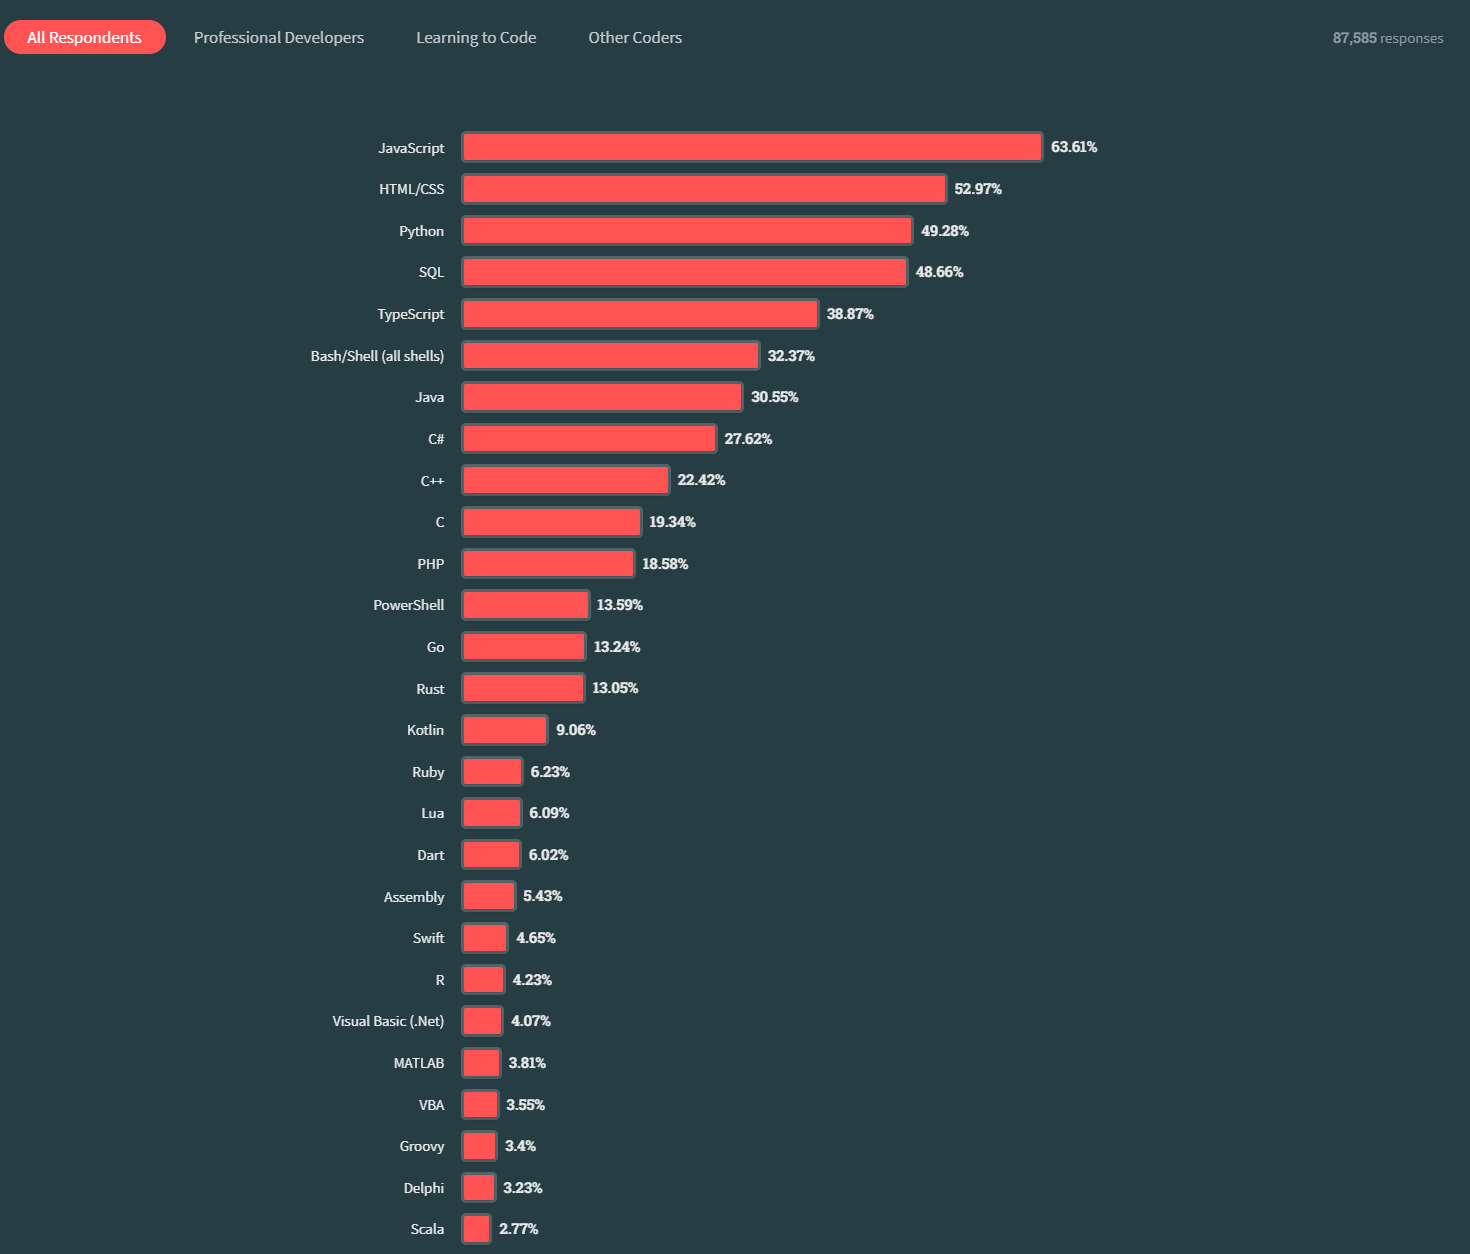
\includegraphics[width=15cm]{images/extrait_sondage_stackoverflow_languages.png}
    %légende
    \caption{Schéma représentant la récupération des données manuellement}
    %label
    \label{fig:schemadonneessauvegarde}
\end{figure}
    
    \subsection{JPEG2000}

JPEG 2000, format présenté en 2000, permet notamment de compresser une image sans perdre la qualité, très utilisé en archives ou en bibliothèques, utilisé à la BnF depuis 2015 pour la numérisation des plans\footnote. Aujourd’hui, plusieurs questions se posent: 
JPEG2000 est supporté que par très peu de navigateur, à des soucis pour s’adapter à l'Open Source et est un format assez complexe\footnote{\textit{Lack of performant open source decoding software}, Open Preservation Foundation, https://wiki.opf-labs.org/display/TR/Lack+of+performant+open+source+decoding+software }.\\ 


En conclusion, concernant les réflexions autour de la durabilité des technologies, tout cela est une question d’arbitrage:\\
\begin{itemize}
    \item Il est possible d’envisager d’utiliser des logiciels Open Source pour éviter le coût financier. De plus, il est plus probable que les technologies open source soient reprises par la communauté.
    \item Possibilité d’estimer la pérennité d’une technologie en fonction de la taille de la communauté. Par exemple, le XML TEI est une grande communauté, notamment avec les guidelines et le TEI consortium, ce qui en fait, comme dit plus haut, un langage pérenne et un choix sûr. Pareil pour le SQL, qui existe depuis presque 50 ans
    \item Le coût des technologies est aussi un critère à prendre en compte, surtout dans le cadre d’un projet aussi long. Maintenance importante aussi quand on utilise des logiciels de niche. \\
    
\end{itemize}


Le choix des technologies à utiliser dans un projet devient très vite un casse-tête, car il faut pouvoir à la fois choisir des logiciels et des langages accessibles aux chercheurs qui n’ont pas spécialement de formation en informatique tout en répondant aux besoins très spécifiques du projet.


    \section{Faire le lien entre les chercheur.se.s et la donnée: UX/UI}

L’user experience (UX) est défini dans la norme ISO 9241-110:2010 comme les perceptions et réponses d’un individu découlant de l’utilisation et/ou la future utilisation d’un produit, d’un système ou d’un service\footnote{User Experience: Challenges and Opportunities}. L’objectif est de prendre en compte les besoins des utilisateurs, ici principalement les chercheur.se.s tout en proposant une interface ergonomique.\\ 
L’user interface (UI) correspond à la façon dont l’utilisateur interagit avec les données. 
L’intérêt de s’intéresser à ces deux notions réside dans la volonté de faire adopter le projet et la plateforme par les utilisateurs. Création d’outils accessibles à un public pas forcément développeur.

    
    \subsection{Interfaces graphiques et outils}

Question des formats de données importants: utiliser des formats faciles à comprendre pour chercheurs, notamment pour export: XML, JSON. Possibilité d’utiliser un format pour le stockage des données et un autre format pour l’export. 
API Rest peuvent être en JSON, en XML, voire même les deux, configurable grâce à l’en-tête HTTP “Accept”. Exemple: “Accept: application/json” ou “Accept: text/xml”. Accès aux données. 

    \subsection{Formats de données}

FAIR: Findable, Accessible, Interoperable, and Re-usable. Mouvement de l’open science, permettre que les données générées pendant la recherche soient réutilisables donc chercheurs encourageant de publier les données des résultats de la recherche\footnote{Francesco Beretta, \textit{A challenge for historical research: Making data FAIR using a collaborative ontology management environment (OntoME)}, in \textit{Semantic Web}, 2021, p279-294.}.
→ guider la production et publication des données issues de la recherche\footnote{Beretta Francesco, \textit{Données ouvertes liées et recherche historique : un changement de paradigme}, 2023, https://journals.openedition.org/revuehn/3349}.
    
    \section{Favoriser la collaboration et l'échange}


    \subsection{API et interopérabilité}

Expérience utilisateur intervient également dans l’expérience du développeur qui implémente l’API: besoin d’être simple à utiliser. Permet également d’assurer que les données soient à jour. API authentification doit se faire avec des formats simples / standardisés (exemple : Basic auth, Bearer Token, Oauth). 
    
    \subsection{Open Data}